\textbf{Pour les exercices \ref{CentreSymAx1} à \ref{CentreSymAx4} :} Trouver l'axe permettant d'obtenir les symétries.
\vspace{-2em}

\begin{minipage}[t]{0.45\textwidth}
    \exo{Raisonner}{CentreSymAx1}
    
    \begin{figure}[H]
        \centering
        \begin{tikzpicture}[scale=0.8]
            \def\mypath{(-2,-2) -- (-1,1) --(-2,0) -- (-1,1.5)--(0,0)--(-2,-2)}
            \draw [white](-3,-3) grid (4,4);
            \draw [thick]\mypath ;
            %\draw (0,-2)--(0,3) node [right]{$(d)$} ;
            \draw [dashed,cm={-1,0,0,1,(0,0)}] \mypath;%Matrice de transformation inverse X et Y 
        \end{tikzpicture}
    \end{figure}
\end{minipage}
\hfill
\begin{minipage}[t]{0.45\textwidth}
    \exo{Raisonner}{CentreSymAx2}
    
    \begin{figure}[H]
        \centering
        \begin{tikzpicture}[scale=0.8]
            \def\mypath{(-3,2) -- (-1,1) --(0,2) -- (1,3)--(0,1)--(-2,2)}
            \draw [thick]\mypath ;
            %\draw (-2,-2)--(3,3) node [right]{$(d)$} ;
            \draw [dashed,cm={0,1,1,0,(0,0)}] \mypath;%Matrice de transformation inverse X et Y
        \end{tikzpicture}
    \end{figure}
\end{minipage}

\begin{minipage}[t]{0.45\textwidth}
    \exo{Raisonner}{CentreSymAx3}
    
    \begin{figure}[H]
        \centering
        \begin{tikzpicture}[scale=0.8]
            \def\mypath{(1,-2) -- (0,-1) --(3,-2) -- (2,-1)--(-1,-1)--(1,-2)}
            \draw [white](-3,-3) grid (4,4);
            \draw [thick]\mypath ;
            %\draw (-2,0)--(3,0) node [right]{$(d)$} ;
            \draw [dashed,cm={0,1,1,0,(0,0)}] \mypath;%Matrice de transformation inverse X et Y
        \end{tikzpicture}
    \end{figure}
\end{minipage}
\hfill
\begin{minipage}[t]{0.45\textwidth}
    \exo{Raisonner}{CentreSymAx4}
    
    \begin{figure}[H]
        \centering
        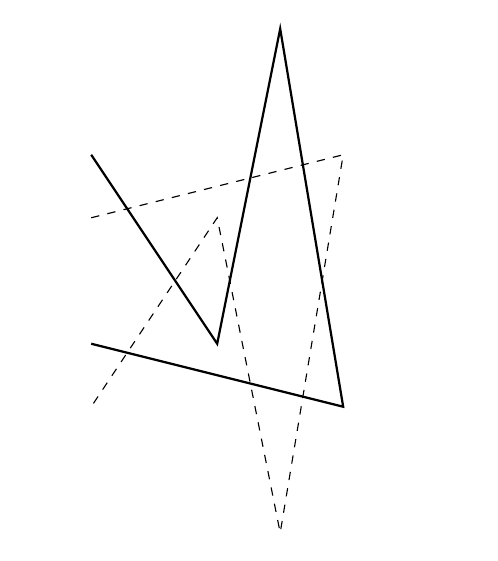
\begin{tikzpicture}[scale=0.8]
            \def\mypath{(-2,-1) -- (2,-2) --(1,4) -- (0,-1)--(-2,2)}
            \draw [white](-3,-3) grid (4,4);
            \draw [thick]\mypath ;
            %\draw (-2,-2)--(3,3) node [right]{$(d)$} ;
            \draw [dashed,cm={1,0,0,-1,(0,0)}] \mypath;%Matrice de transformation inverse X et Y
        \end{tikzpicture}
    \end{figure}
\end{minipage}

\textbf{Pour les exercices \ref{CentreSymCent1} à \ref{CentreSymCent4} :} Trouver le centre qui permet les symétrie centrales suivantes.

\begin{minipage}[t]{0.45\textwidth}
    \exo{Représenter}{CentreSymCent1}
    
    \begin{figure}[H]
        \centering
        \begin{tikzpicture}[scale=0.8]
            \tikzset{
                homothety at/.style args={#1 scaled by #2}{shift={($(#1)!#2!(0,0)$)},scale=#2},}
            \def\mypath{(-2,-2) -- (-1,1) --(-2,0) -- (-1,1.5)--(0,0)--(-2,-2)}
            \draw [white](-3,-3) grid (4,4);
            \fill[white] (0,0) coordinate (c) circle(2pt) node [above] {$O$};
            \draw [thick]\mypath ;
            \begin{scope}[homothety at=c scaled by -1]
                \draw [dashed]\mypath;
            \end{scope}
        \end{tikzpicture}
    \end{figure}
\end{minipage}
\hfill
\begin{minipage}[t]{0.45\textwidth}
    \exo{Représenter}{CentreSymCent2}
    
    \begin{figure}[H]
        \centering
        \begin{tikzpicture}[scale=0.8]
            \tikzset{
                homothety at/.style args={#1 scaled by #2}{shift={($(#1)!#2!(0,0)$)},scale=#2},}
            \def\mypath{(-3,2) -- (-1,1) --(0,2) -- (1,3)--(0,1)--(-2,2)}
            \fill[white] (1,0) coordinate (c) circle(2pt) node [above] {$O$};
            \draw [white](-3,-3) grid (4,4);
            \draw [thick]\mypath ;
            \begin{scope}[homothety at=c scaled by -1]
                \draw[dashed] \mypath;
            \end{scope}
        \end{tikzpicture}
    \end{figure}
\end{minipage}

\begin{minipage}[t]{0.45\textwidth}
    \exo{Représenter}{CentreSymCent3}
    
    \begin{figure}[H]
        \centering
        \begin{tikzpicture}[scale=0.8]
            \tikzset{
                homothety at/.style args={#1 scaled by #2}{shift={($(#1)!#2!(0,0)$)},scale=#2},}
            \def\mypath{(1,-2) -- (0,-1) --(3,-2) -- (2,-1)--(-1,-1)--(1,-2)}
            \fill [white](0,0) coordinate (c) circle(2pt) node [above] {$O$};
            \draw [white](-3,-3) grid (4,4);
            \draw [thick]\mypath ;
            \begin{scope}[homothety at=c scaled by -1]
                \draw [dashed]\mypath;
            \end{scope}
        \end{tikzpicture}
    \end{figure}
\end{minipage}
\hfill
\begin{minipage}[t]{0.45\textwidth}
    \exo{Représenter}{CentreSymCent4}
    
    \begin{figure}[H]
        \centering
        \begin{tikzpicture}[scale=0.8]
            \tikzset{
                homothety at/.style args={#1 scaled by #2}{shift={($(#1)!#2!(0,0)$)},scale=#2},}
            \def\mypath{(-2,-1) -- (2,-2) --(1,4) -- (0,-1)--(-2,2)}
            \fill [white](0,1) coordinate (c) circle(2pt) node [above] {$O$};
            \draw [white](-3,-3) grid (4,4);
            \draw [thick]\mypath ;
            \begin{scope}[homothety at=c scaled by -1]
                \draw [dashed]\mypath;
            \end{scope}
        \end{tikzpicture}
    \end{figure}
\end{minipage}

\newpage
\textbf{Pour les exercices \ref{CentreRota1} à \ref{CentreRota4} :} Trouver le centre et l'angle  des rotations suivantes.
\vspace{-2em}

\begin{minipage}[t]{0.45\textwidth}
    \exo{Représenter}{CentreRota1}
        
    \begin{figure}[H]
        \centering
        \begin{tikzpicture}[scale=0.8]
            \def\mypath{(-2,-2) -- (-1,1) --(-2,0) -- (-1,1.5)--(0,0)--(-2,-2)}
            \fill[white] (0,0) coordinate (c) circle(2pt) node [above] {$0$};
            \draw [white](-3,-3) grid (4,4);
            \draw [thick]\mypath ;
            \draw [dashed,rotate=-160] \mypath ;
        \end{tikzpicture}
    \end{figure}
\end{minipage}
\hfill
\begin{minipage}[t]{0.45\textwidth}
    \exo{Représenter}{CentreRota2}
        
    \begin{figure}[H]
        \centering
        \begin{tikzpicture}[scale=0.8]
            \def\mypath{(-3,2) -- (-1,1) --(0,2) -- (1,3)--(0,1)--(-2,2)}
            \fill[white] (0,0) coordinate (c) circle(2pt) node [above] {$0$};
            \draw [white](-3,-3) grid (4,4);
            \draw [thick]\mypath ;
            \draw [dashed,rotate=30] \mypath ;
        \end{tikzpicture}
    \end{figure}
\end{minipage}

\begin{minipage}[t]{0.45\textwidth}
    \exo{Représenter}{CentreRota3}
        
    \begin{figure}[H]
        \centering
        \begin{tikzpicture}[scale=0.8]
            \def\mypath{(1,-2) -- (0,-1) --(3,-2) -- (2,-1)--(-1,-1)--(1,-2)}
            \fill[white] (0,0) coordinate (c) circle(2pt) node [above] {$0$};
            \draw [white](-3,-3) grid (4,4);
            \draw [thick]\mypath ;
            \draw [dashed,rotate=-75] \mypath ;
        \end{tikzpicture}
    \end{figure}
\end{minipage}
\hfill
\begin{minipage}[t]{0.45\textwidth}
    \exo{Représenter}{CentreRota4}
        
    \begin{figure}[H]
        \centering
        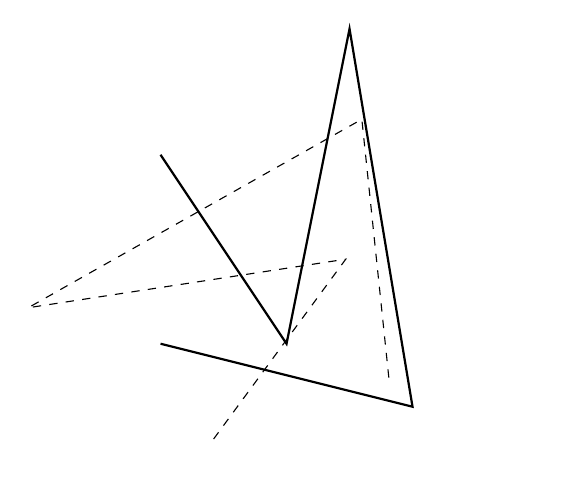
\begin{tikzpicture}[scale=0.8]
            \def\mypath{(-2,-1) -- (2,-2) --(1,4) -- (0,-1)--(-2,2)}
            \fill[white] (0,0) coordinate (c) circle(2pt) node [above] {$0$};
            \draw [white](-3,-3) grid (4,4);
            \draw [thick]\mypath ;
            \draw [dashed,rotate=110] \mypath ;
        \end{tikzpicture}
    \end{figure}
\end{minipage}
\vspace{1em}
\textbf{Pour les exercices \ref{CentreHomot1} à \ref{CentreHomot4} :}Trouver le centre et le rapport des homotéties suivantes.
\vspace{-2em}

\begin{minipage}[t]{0.45\textwidth}
    \exo{Représenter}{CentreHomot1}
        
    \begin{figure}[H]
        \centering
        \begin{tikzpicture}[scale=0.8]
            \tikzset{
                homothety at/.style args={#1 scaled by #2}{shift={($(#1)!#2!(0,0)$)},scale=#2},}
            \fill[white] (-1,-1) coordinate (c) circle(2pt) node [above] {$O$};
            \def\mypath{(-2,-2) -- (-1,1) --(-2,0) -- (-1,1.5)--(0,0)--(-2,-2)}
            \draw [white](-3,-3) grid (5,5);
            \draw [thick]\mypath ;
            \begin{scope}[homothety at=c scaled by 2]
                \draw[dashed] \mypath;
            \end{scope}
        \end{tikzpicture}
    \end{figure}
\end{minipage}
\hfill
\begin{minipage}[t]{0.45\textwidth}
    \exo{Représenter}{CentreHomot2}
        
    \begin{figure}[H]
        \centering
        \begin{tikzpicture}[scale=0.8]
            \tikzset{
                homothety at/.style args={#1 scaled by #2}{shift={($(#1)!#2!(0,0)$)},scale=#2},}
            \def\mypath{(-3,2) -- (-1,1) --(0,2) -- (1,3)--(0,1)--(-2,2)}
            \draw [white](-3,-3) grid (5,5);
            \draw [thick]\mypath ;
            \fill[white] (0,-2) coordinate (c) circle(2pt) node [above] {$O$};
            \begin{scope}[homothety at=c scaled by 0.75]
                \draw[dashed] \mypath;
            \end{scope}
        \end{tikzpicture}
    \end{figure}
\end{minipage}

\begin{minipage}[t]{0.45\textwidth}
    \exo{Représenter}{CentreHomot3}
        
    \begin{figure}[H]
        \centering
        \begin{tikzpicture}[scale=0.8]
            \tikzset{
                homothety at/.style args={#1 scaled by #2}{shift={($(#1)!#2!(0,0)$)},scale=#2},}
            \def\mypath{(-1,-2) -- (0,-1) --(3,-2) -- (2,0)--(-1,-3)--(-1,-2)}
            \draw [white](-3,-3) grid (5,5);
            \draw [thick]\mypath ;
            \fill[white] (1,0) coordinate (c) circle(2pt) node [above] {$O$};
            \begin{scope}[homothety at=c scaled by -2]
                \draw[dashed] \mypath;
            \end{scope}
        \end{tikzpicture}
    \end{figure}
\end{minipage}
\hfill
\begin{minipage}[t]{0.45\textwidth}
    \exo{Représenter}{CentreHomot4}
        
    \begin{figure}[H]
        \centering
        \begin{tikzpicture}[scale=0.8]
            \tikzset{
                homothety at/.style args={#1 scaled by #2}{shift={($(#1)!#2!(0,0)$)},scale=#2},}
            \def\mypath{(-1,-1) -- (2,-2) --(1,3) -- (0,-1)--(-1,2)}
            \draw [white](-3,-3) grid (5,5);
            \draw [thick]\mypath ;
            \fill[white] (2,1) coordinate (c) circle(2pt) node [above] {$O$};
            \begin{scope}[homothety at=c scaled by 1.5]
                \draw[dashed] \mypath;
            \end{scope}
        \end{tikzpicture}
    \end{figure}
\end{minipage}